\documentclass[aspectratio=169,11pt]{beamer}
\usetheme{Madrid}
\usecolortheme{default}
\usepackage{booktabs}
\usepackage{tikz}
\usepackage{xcolor}
\usepackage{graphicx}
\usepackage{array}

% Custom colors
\definecolor{critred}{RGB}{204,0,0}
\definecolor{warnorg}{RGB}{230,120,0}
\definecolor{okgreen}{RGB}{0,153,0}
\definecolor{lightgray}{RGB}{230,230,230}
\definecolor{codebg}{RGB}{245,245,245}

% Remove navigation symbols
\setbeamertemplate{navigation symbols}{}

% Smaller footnote size
\setbeamerfont{footnote}{size=\tiny}

\title{Referee Report --- Round 5}
\subtitle{Tennis Match Simulator}
\author{Referee 2}
\date{2026-02-09}

\begin{document}

% =============================================================================
% SLIDE 1: Title
% =============================================================================
\begin{frame}
\titlepage
\end{frame}

% =============================================================================
% SLIDE 2: Executive Summary
% =============================================================================
\begin{frame}{Critical Data Leakage Invalidates All Backtest Results}

\textbf{Verdict:} \textcolor{critred}{\textbf{Major Revisions Required}}

\vspace{0.8em}

\begin{itemize}
  \item \textcolor{critred}{\textbf{CRITICAL:}} ATP match data uses \textbf{tournament start dates}; betting data uses \textbf{actual match dates}
  \item Later-round results leak into Elo ratings when predicting earlier rounds
  \item The existing leakage check (\texttt{validate\_elo\_betting.R}) is \textbf{tautological} --- it checks \texttt{tourney\_date} against \texttt{tourney\_date}
  \item All reported metrics (68.6\% accuracy, +9.9pp over MC, ROI figures) are unreliable
\end{itemize}

\vspace{0.8em}

\textbf{Note:} The Elo implementation itself is correct. The bug is in how historical match dates are defined, not in the model.

\end{frame}

% =============================================================================
% SLIDE 3: The Date Mismatch
% =============================================================================
\begin{frame}[t]{Two Data Sources Use Different Date Semantics}

\begin{table}
\centering
\small
\begin{tabular}{lllp{5.0cm}}
\toprule
\textbf{Source} & \textbf{Column} & \textbf{Semantics} & \textbf{Brisbane 2024 Example} \\
\midrule
ATP (Sackmann) & \texttt{tourney\_date} & Tournament start & All 31 matches: \texttt{2024-01-01} \\
\addlinespace[3pt]
Betting (t-d.co.uk) & \texttt{Date} & Actual match date & R1: Dec 31, QF: Jan 3, F: Jan~4 \\
\bottomrule
\end{tabular}
\end{table}

\vspace{0.5em}

\textbf{In the code:}
\begin{itemize}
  \item \texttt{02\_player\_stats.R:68} --- \texttt{match\_date = ymd(tourney\_date)}
  \item \texttt{05\_betting\_data.R:316} --- \texttt{match\_date = as\_date(match\_date)}
\end{itemize}

\vspace{0.5em}
Both are stored as \texttt{match\_date} in their respective data frames --- same name, different~semantics.

\end{frame}

% =============================================================================
% SLIDE 4: The Leakage Mechanism
% =============================================================================
\begin{frame}{How Future Results Leak Into Predictions}

\begin{columns}
\column{0.55\textwidth}

\textbf{Predicting a QF on Jan 3:}

\begin{enumerate}
  \item Betting data: \texttt{cutoff = Jan 3}
  \item ATP filter: \texttt{tourney\_date < Jan 3}
  \item Tournament started Jan 1 $\rightarrow$ \textbf{passes filter}
  \item \textcolor{critred}{\textbf{SF (Jan 3) and Final (Jan 4) included in Elo}}
\end{enumerate}

\vspace{0.5em}
The model knows who won the Final before predicting the Quarterfinal.

\column{0.42\textwidth}

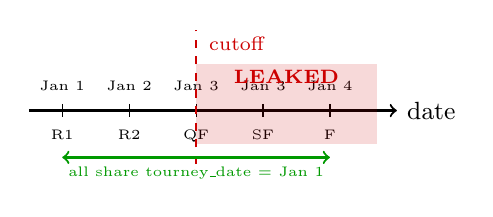
\begin{tikzpicture}[scale=0.85]
  % Timeline
  \draw[thick,->] (0,0) -- (5.5,0) node[right] {\small date};

  % Tournament dates
  \foreach \x/\label/\round in {0.5/Jan 1/R1, 1.5/Jan 2/R2, 2.5/Jan 3/QF, 3.5/Jan 3/SF, 4.5/Jan 4/F} {
    \draw (\x,0.1) -- (\x,-0.1);
    \node[above,font=\tiny] at (\x,0.15) {\label};
    \node[below,font=\tiny] at (\x,-0.15) {\round};
  }

  % Cutoff line
  \draw[critred,thick,dashed] (2.5,-0.8) -- (2.5,1.2);
  \node[critred,font=\scriptsize,right] at (2.55,1.0) {cutoff};

  % Leaked region
  \fill[critred,opacity=0.15] (2.5,-0.5) rectangle (5.2,0.7);
  \node[critred,font=\scriptsize] at (3.85,0.5) {\textbf{LEAKED}};

  % tourney_date
  \draw[okgreen,thick,<->] (0.5,-0.7) -- (4.5,-0.7);
  \node[okgreen,font=\tiny,below] at (2.5,-0.7) {all share tourney\_date = Jan 1};
\end{tikzpicture}

\end{columns}

\end{frame}

% =============================================================================
% SLIDE 5: The Tautological Validation
% =============================================================================
\begin{frame}{Existing Leakage Check Tests the Wrong Thing}

\texttt{validate\_elo\_betting.R:46--62}:

\vspace{0.3em}

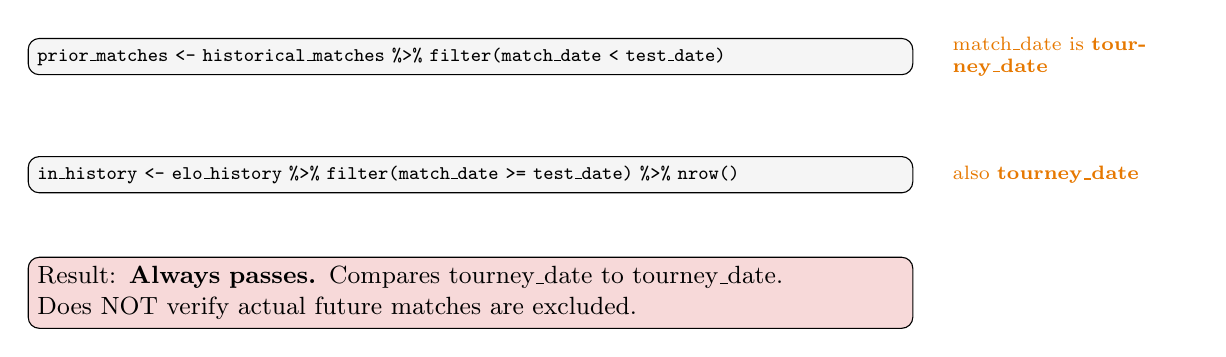
\begin{tikzpicture}
  % Step 1
  \node[draw,rounded corners,fill=codebg,text width=11cm,font=\ttfamily\scriptsize] at (0,2.5) {
    prior\_matches <- historical\_matches \%>\% filter(match\_date < test\_date)
  };
  \node[right,font=\scriptsize,text width=3cm] at (6,2.5) {\textcolor{warnorg}{match\_date is \textbf{tourney\_date}}};

  % Step 2
  \node[draw,rounded corners,fill=codebg,text width=11cm,font=\ttfamily\scriptsize] at (0,1.0) {
    in\_history <- elo\_history \%>\% filter(match\_date >= test\_date) \%>\% nrow()
  };
  \node[right,font=\scriptsize,text width=3cm] at (6,1.0) {\textcolor{warnorg}{also \textbf{tourney\_date}}};

  % Verdict
  \node[draw,rounded corners,fill=critred!15,text width=11cm,font=\small] at (0,-0.5) {
    Result: \textbf{Always passes.} Compares tourney\_date to tourney\_date. \\
    Does NOT verify actual future matches are excluded.
  };
\end{tikzpicture}

\end{frame}

% =============================================================================
% SLIDE 6: Impact Quantification
% =============================================================================
\begin{frame}{Leakage Disproportionately Inflates Elo Accuracy}

\begin{columns}
\column{0.48\textwidth}

\textbf{Why Elo is more affected than MC:}
\begin{itemize}
  \item Each leaked match changes Elo by up to $\pm$32 points (K-factor)
  \item Effect compounds across multiple leaked rounds
  \item Players who advance get rating boosts from future wins
  \item Those players \emph{did win} their earlier matches $\rightarrow$ spurious accuracy
\end{itemize}

\column{0.48\textwidth}

\textbf{Why MC is less affected:}
\begin{itemize}
  \item Serve/return stats aggregated over 9 years (2015+)
  \item A few extra matches barely change averages
  \item No per-match compounding effect
  \item Leakage has minimal impact on MC predictions
\end{itemize}

\end{columns}

\vspace{0.5em}

\begin{table}
\centering
\small
\begin{tabular}{lccc}
\toprule
\textbf{Tournament Type} & \textbf{Matches} & \textbf{Max Gap} & \textbf{R1+R2 (\% of draw)} \\
\midrule
Grand Slam & $\sim$127 & 14 days & 75\% \\
Masters 1000 & $\sim$55--95 & 7--9 days & 75\% \\
ATP 500 / 250 & $\sim$31 & 6 days & 75\% \\
\bottomrule
\end{tabular}
\end{table}

\end{frame}

% =============================================================================
% SLIDE 7: Reported Metrics Are Unreliable
% =============================================================================
\begin{frame}{All Reported Metrics Are Based on Leaked Data}

\begin{table}
\centering
\begin{tabular}{lcl}
\toprule
\textbf{Metric} & \textbf{Reported Value} & \textbf{Status} \\
\midrule
Elo Accuracy & 68.6\% & \textcolor{critred}{Unreliable --- leakage inflated} \\
MC Accuracy & 58.7\% & \textcolor{warnorg}{Less affected but same bug} \\
Elo -- MC Gap & +9.9 pp & \textcolor{critred}{Unreliable --- differential leakage} \\
Brier Score (Elo) & 0.2029 & \textcolor{critred}{Unreliable} \\
Log Loss (Elo) & 0.5913 & \textcolor{critred}{Unreliable} \\
All ROI / Edge figures & Various & \textcolor{critred}{Unreliable} \\
\bottomrule
\end{tabular}
\end{table}

\vspace{0.8em}

\textbf{Conservative estimate:} Leakage inflates Elo accuracy by 1.3--2.2 percentage points. The true Elo--MC gap may be 8--9 pp instead of 9.9 pp --- or could be smaller if the Elo model's calibration is also affected.

\vspace{0.5em}
\textit{True performance can only be determined after fixing the date alignment.}

\end{frame}

% =============================================================================
% SLIDE 8: Elo Implementation Is Sound
% =============================================================================
\begin{frame}{Elo Implementation Itself Is Correct (Modulo Dates)}

\begin{columns}
\column{0.48\textwidth}

\textcolor{okgreen}{\checkmark} Standard Elo formula \\
\textcolor{okgreen}{\checkmark} Per-player K-factors (fixed R3) \\
\textcolor{okgreen}{\checkmark} Surface-specific blending \\
\textcolor{okgreen}{\checkmark} Alphabetical ordering (no calibration bias) \\
\textcolor{okgreen}{\checkmark} 14 unit tests passing \\
\textcolor{okgreen}{\checkmark} History tracking (fixed R4) \\

\column{0.48\textwidth}

\textcolor{warnorg}{?} K=32 not validated for tennis \\
\textcolor{warnorg}{?} Scale factor 400 not validated \\
\textcolor{warnorg}{?} No calibration analysis published \\
\textcolor{warnorg}{?} No decay for inactive players \\
\textcolor{warnorg}{?} Surface Elo starts at 1500 \\

\end{columns}

\vspace{1em}

The Elo module is well-structured, well-tested code. The issue is upstream: the date field fed into it is semantically wrong.

\end{frame}

% =============================================================================
% SLIDE 9: Edge Analysis Assessment
% =============================================================================
\begin{frame}{Edge Analysis: Methodology Sound, Inputs Compromised}

\textbf{What is correct:}
\begin{itemize}
  \item Edge = model\_prob $-$ implied\_prob (includes vig --- correct for betting decisions)
  \item Fractional Kelly criterion with 5\% max bet cap
  \item Bootstrap CI for ROI (1,000 resamples)
  \item Four baseline strategies compared
\end{itemize}

\vspace{0.5em}

\textbf{What is problematic:}
\begin{itemize}
  \item \textcolor{critred}{All edge calculations use leaked model probabilities}
  \item No out-of-sample test completed (H2 2024 data unavailable)
  \item Closing vs.\ opening odds not formally verified from source documentation
  \item \texttt{validate\_elo\_betting.R} results not reported in any correspondence round
\end{itemize}

\vspace{0.5em}

\textbf{Bottom line:} The edge analysis framework is well-designed. But the inputs (model probabilities) are contaminated by leakage, making all ROI figures uninterpretable.

\end{frame}

% =============================================================================
% SLIDE 10: Replication Readiness
% =============================================================================
\begin{frame}{Replication Readiness: 7/10 (decreased from 8/10)}


\begin{tikzpicture}
  % Progress bar
  \fill[okgreen!60] (0,0) rectangle (7,0.5);
  \fill[gray!30] (7,0) rectangle (10,0.5);
  \node[font=\bfseries] at (5,0.25) {7/10};
\end{tikzpicture}

\vspace{0.8em}

\begin{columns}
\column{0.48\textwidth}
\textcolor{okgreen}{\checkmark} Folder structure \\
\textcolor{okgreen}{\checkmark} Relative paths \\
\textcolor{okgreen}{\checkmark} Variable naming \\
\textcolor{okgreen}{\checkmark} Script naming / ordering \\
\textcolor{okgreen}{\checkmark} Dependencies (\texttt{renv.lock}) \\
\textcolor{okgreen}{\checkmark} Random seeds set \\
\textcolor{okgreen}{\checkmark} Master script exists \\

\column{0.48\textwidth}
\textcolor{critred}{\texttimes} Date alignment broken (results unreliable) \\
\textcolor{warnorg}{\texttimes} Comparison scripts not in master pipeline \\
\textcolor{warnorg}{\texttimes} In-text statistics manually entered \\

\end{columns}

\vspace{0.5em}
\footnotesize Decreased from 8/10 because biased results are not meaningfully replicable.

\end{frame}

% =============================================================================
% SLIDE 11: Recommendations
% =============================================================================
\begin{frame}{Recommendations (Priority Order)}

\begin{enumerate}
  \item \textcolor{critred}{\textbf{Fix date alignment}} --- Replace \texttt{tourney\_date} with actual match dates
    \begin{itemize}
      \footnotesize
      \item Preferred: Join ATP matches with betting data by player names + tournament
      \item Alternative: Infer from \texttt{round} column (R1 = day 1, R2 = day 2, etc.)
      \item Stopgap: Use 14-day buffer (\texttt{cutoff - 14d}) to bound leakage
    \end{itemize}

  \item \textcolor{critred}{\textbf{Fix leakage validation}} --- Test against actual match dates, not tournament dates

  \item \textcolor{warnorg}{\textbf{Re-run all backtests}} with corrected dates; update CLAUDE.md

  \item \textcolor{warnorg}{\textbf{Quantify leakage impact}} --- Compare accuracy before/after fix

  \item Report Elo calibration (predicted vs.\ actual win rates by bin)

  \item Add McNemar test for model comparison significance

  \item K-factor sensitivity analysis (K = 16, 20, 24, 32, 40)
\end{enumerate}

\end{frame}

\end{document}
